Используемые формулы в построении фигуры.

Расчет шага \(\alpha\): \[360/n\] Получение n-угольника:
\[T_n = (r*cos(\alpha)+center_x;r*sin(\alpha)+center_y),\]

Для поворота фигур была использована матрица поворота.
\[ \begin{array}{ccc}
x' = x*cos(\alpha)-y*sin(\alpha),
\\
y' = x*sin(\alpha)+y*cos(\alpha).
\end{array}
\] Формула зависимости массива brushColors{[}5{]} от угла поворота.
\[(((i+1)*250+\alpha/10)\%359;(i*150)\%255;150)_{HSL}\]

Формулы для радиусов вписанных в треугольник a окружностей. \[
    \begin{array}{ccc}
    r_1 = (height-20|width-20)/20
    \\
    r_2 = r_1+(height-30|width-30)
    \\
    r_3 = r_2+(height-30|width-30)
    \end{array}
\]

Сторона a вычисляется по радиусу наибольшей вписанной в него окружности.
\[a = 2*\sqrt{3}*r_3\] Радиус описанной окружности треугольника a.
\[R_a = \frac{\sqrt{3}*a}{3}\]

Окружности на ходящиеся на вершинах треугольника находятся на вершинах
скрытого треугольника a' с радиусом описанной окружности на a/8 больше
чем у треугольника a. \[R_{a'} = R_a+\frac{a}{8} \]

\hypertarget{ux43eux43aux43dux43e-ux43fux440ux43eux433ux440ux430ux43cux43cux44b}{%
\subsubsection{Окно
программы}\label{ux43eux43aux43dux43e-ux43fux440ux43eux433ux440ux430ux43cux43cux44b}}

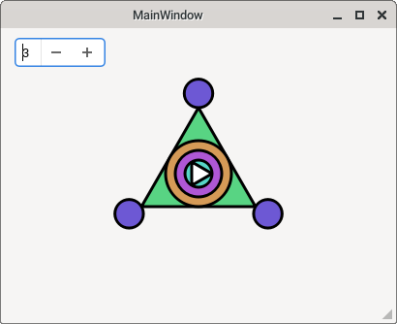
\includegraphics{./files/pic2.png}
